% !TeX root = ../main.tex
\chapter*{3. Results}
\setcounter{chapter}{3}
\addcontentsline{toc}{chapter}{3. Results}
\section{Summary of the simulated data}
\noindent
Overall, we had 17,500 samples from 18 replicates of metacommunity with 975 scenarios (5 competition types, 15 dispersal ability types and 13 niche widths) generated by \citeauthor{thompson2020process}'s framework. Each sample contained 20 snapshots of the species composition at different time steps. After filtering out the incomplete samples, which missed some summary statistics, we retained 5983 samples and 399 scenarios and used them in further analysis.

The parametric space for the retained samples was shown by heat map (Fig. \ref{fig:para}). The scenarios with weak dispersal ability $a$ and narrow niche width $\lambda$ were mostly filtered out. Parametric space defined by dispersal ability $a$ and niche width $\lambda$ was wider in scenarios of no competition, stable competition and equal competition (Fig. \ref{fig:para-no}, \ref{fig:para-stable}, \ref{fig:para-equal}), compared to mixed competition and competition-colonization trade-off (Fig. \ref{fig:para-mixed}, \ref{fig:para-CC}). We defined four metacommunity archetypes based on the parametric space (Fig. \ref{fig:para-arch}).

%
\begin{figure}
	\centering
	\begin{subfigure}[b]{0.45\linewidth}
		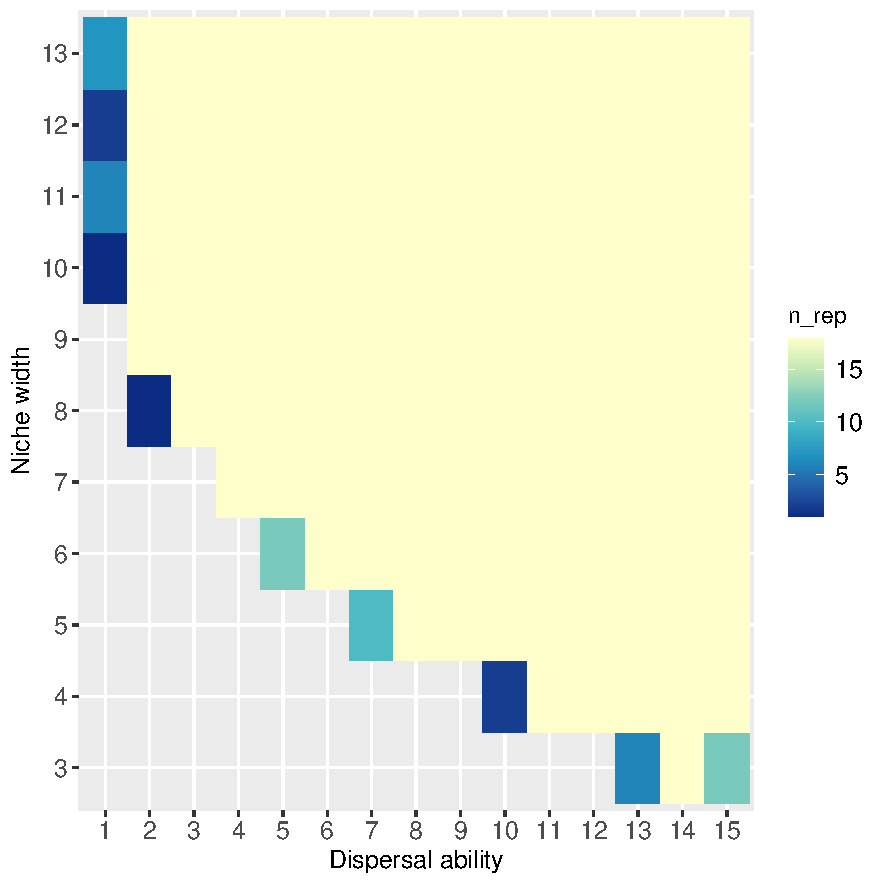
\includegraphics[width=\linewidth]{./figures/Parameter_space_overlook_no_competition.pdf}
		\caption{No competition}
		\label{fig:para-no}
	\end{subfigure}
	\begin{subfigure}[b]{0.45\linewidth}
		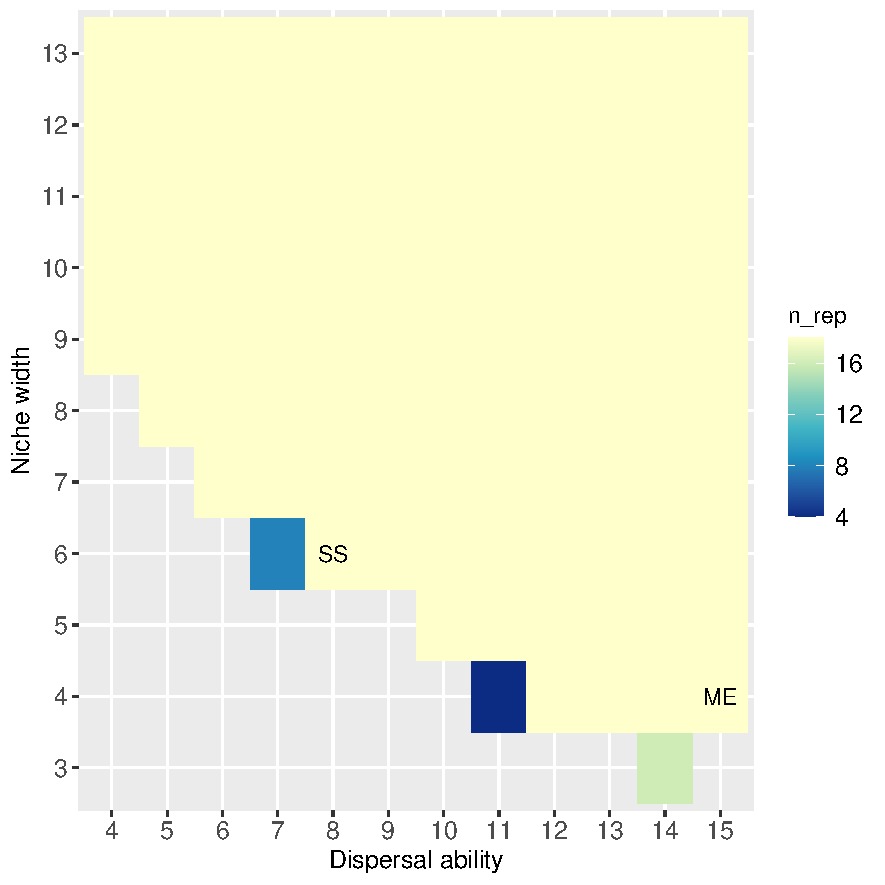
\includegraphics[width=\linewidth]{./figures/Parameter_space_overlook_stable_competition.pdf}
		\caption{Stable competition}
		\label{fig:para-stable}
	\end{subfigure}
	\begin{subfigure}[b]{0.45\linewidth}
		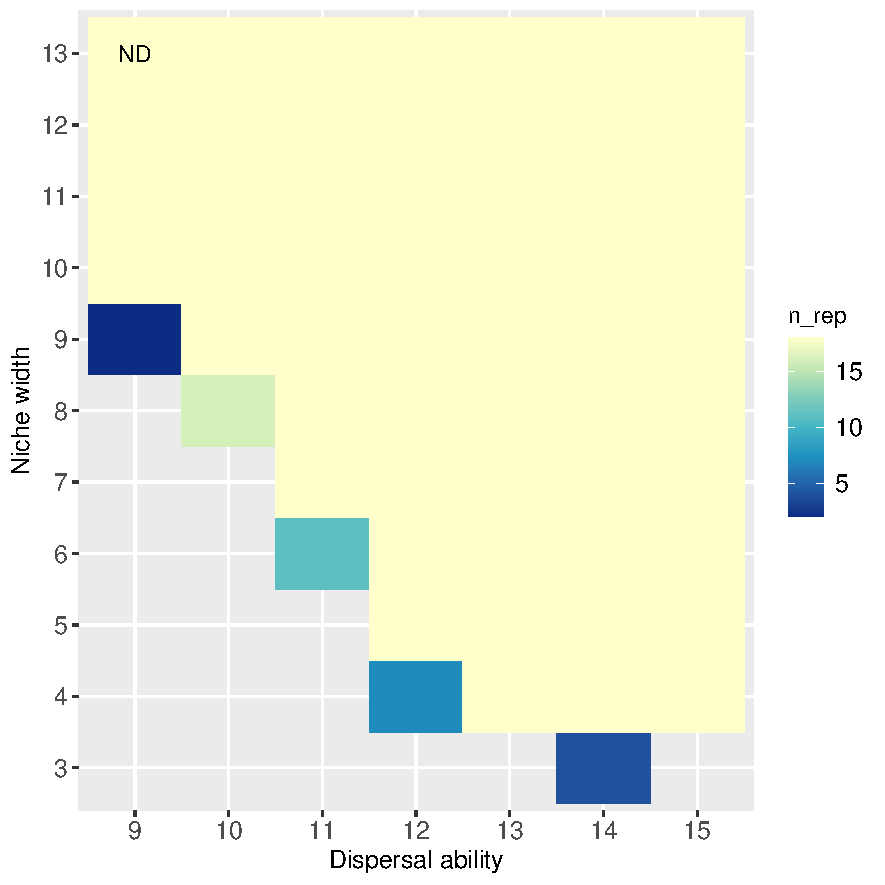
\includegraphics[width=\linewidth]{./figures/Parameter_space_overlook_equal_competition.pdf}
		\caption{Equal competition}
		\label{fig:para-equal}
	\end{subfigure}
	\begin{subfigure}[b]{0.45\linewidth}
		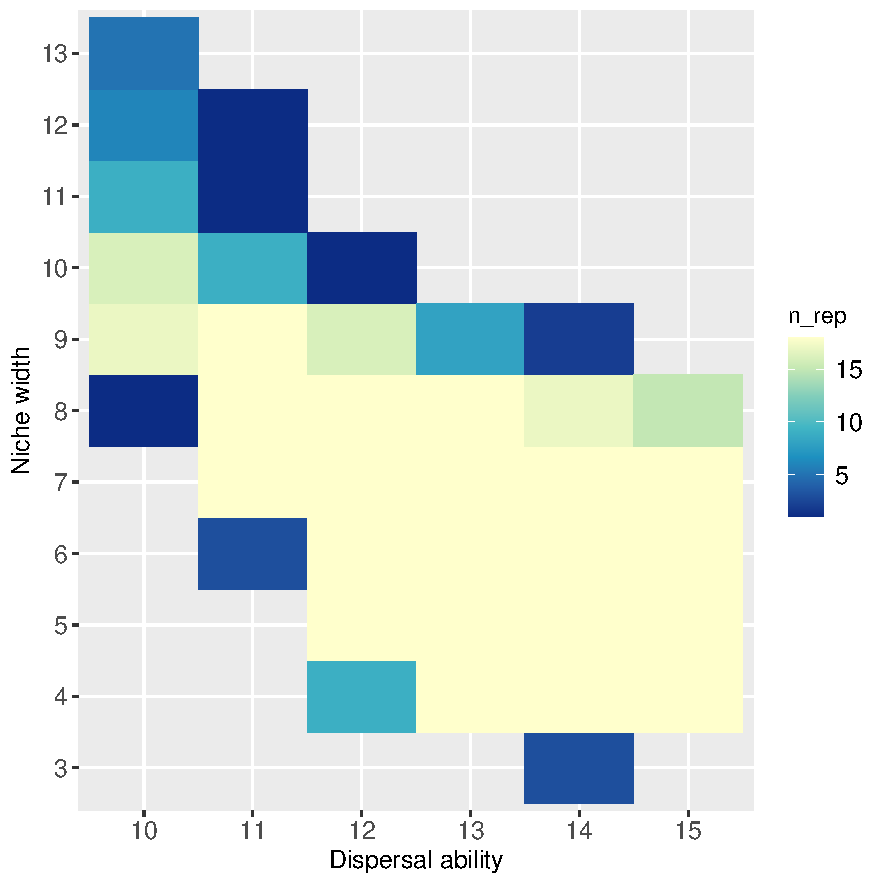
\includegraphics[width=\linewidth]{./figures/Parameter_space_overlook_mixed_competition.pdf}
		\caption{mixed competition}
		\label{fig:para-mixed}
	\end{subfigure}
\end{figure}
\begin{figure}\ContinuedFloat
	\centering
	\begin{subfigure}[b]{0.45\linewidth}
		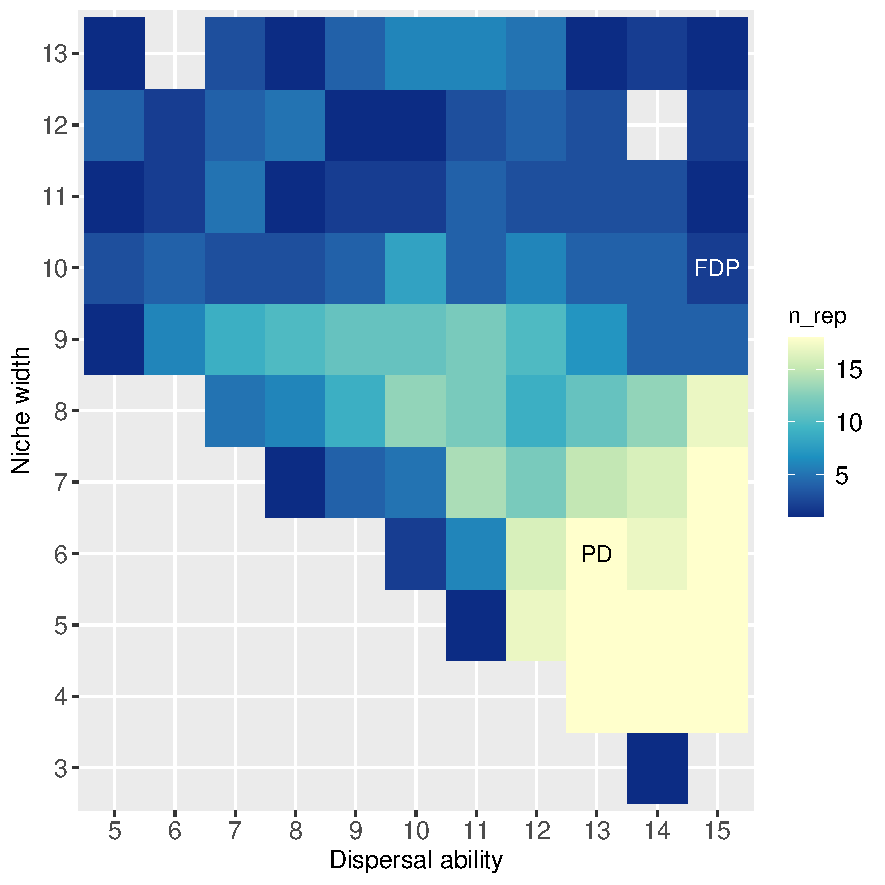
\includegraphics[width=\linewidth]{./figures/Parameter_space_overlook_CC_tradeoff.pdf}
		\caption{CC trade-off}
		\label{fig:para-CC}
	\end{subfigure}
	\begin{subfigure}[b]{0.45\linewidth}
		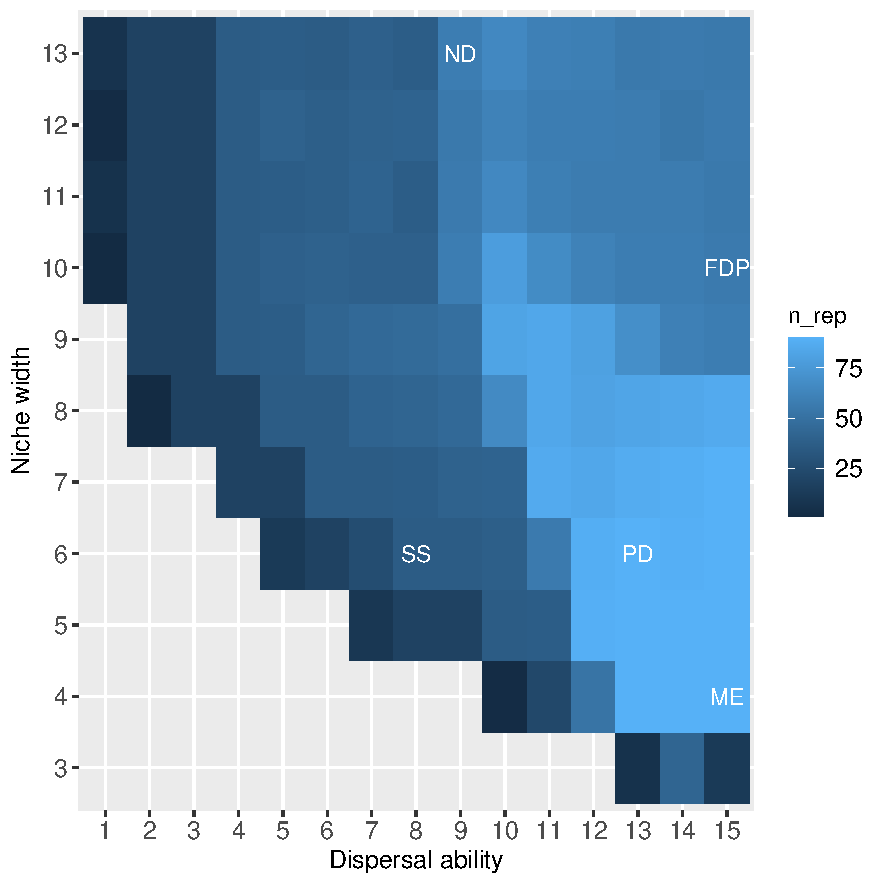
\includegraphics[width=\linewidth]{./figures/Parameter_space_overlook_archetypes.pdf}
		\caption{Archetypes}
		\label{fig:para-arch}
	\end{subfigure}
	\caption[Parametric space defined by niche width, dispersal ability and competition type.]{\small
		Parametric space defined by niche width, dispersal ability and competition type. The number on the two axes represents the level of the niche width and dispersal ability. On the x-axis, the numbers from 1 to 15 are the dispersal ability from weak to strong. On the y-axis, the numbers from 1 to 13 are the niche widths from narrow to wide. The values in the tile plots represent the number of replicates that remain after excluding those with too low species abundance, diversity and occurrence, or those too sparse to calculate DNCI. If the scenario has no replicates after filtering, the values are shown as missing in the tile plots. The axes are truncated since no replicates remained after data filtering for those scenarios. Panels (a)-(e) show the parameter space defined by niche width and dispersal ability with different competition types. Panel (f) is the summation of the five tile plots from (a) to (e). The labels in the tile plot show the subjective definition of the four metacommunity archetypes in the parametric space: \textit{species sorting} (SS), \textit{neutral dynamics} (ND), \textit{mass effect} (ME) and \textit{patch dynamics} (PD). The species in the Fushan Forest Dynamics Plot (FDP) are predicted to interact with each other with competition-colonization trade-off, average strong dispersal ability and wide niches.}
	\label{fig:para}
\end{figure}
%

\section{Summary statistics of the simulated metacommunity}
\noindent
Statistics of beta-diversity variation partitioning, DNCI and Stegen's framework were calculated for the remaining 5983 samples. All the statistics fluctuated across time and differed between replicates (Fig. \ref{fig:stat_comp}). The summary statistics derived from Stegen's frame could successfully separate the four archetypes. The relative importance of selection could separate SS and ND from each other; the relative importance of homogenizing dispersal could separate ME and ND; the relative importance of drift could separate PD and SS. In beta-diversity variation partitioning, only ND could be separated from the other archetypes based on unexplained variation. DNCI could not identify any archetypes.

The ranges of the summary statistics of three analytical methods were calculated (Tab. \ref{tbl:sum_stat}). The reason that the minimal value of the variation explained only by environment, only by space, and by both environment and space derived from the variation partitioning was negative was that the explained variation was calculated by the adjusted R$^2$ which may be negative when R$^2$ is extremely close to zero \citep[pp.~633]{legendre2012numerical}. The maximum value of residual derived from variation partitioning could be larger than 1 because the residual was calculated by 1 minus the sum of the explained variation by either environment or space. The statistics derived from Stegen's framework ranged from 0 to 1. DNCI and its standard deviation had no boundary limitation. The average and standard deviation were also calculated for each summary statistic.

% figure: comparing different archetypes
\begin{figure}
	\centering
	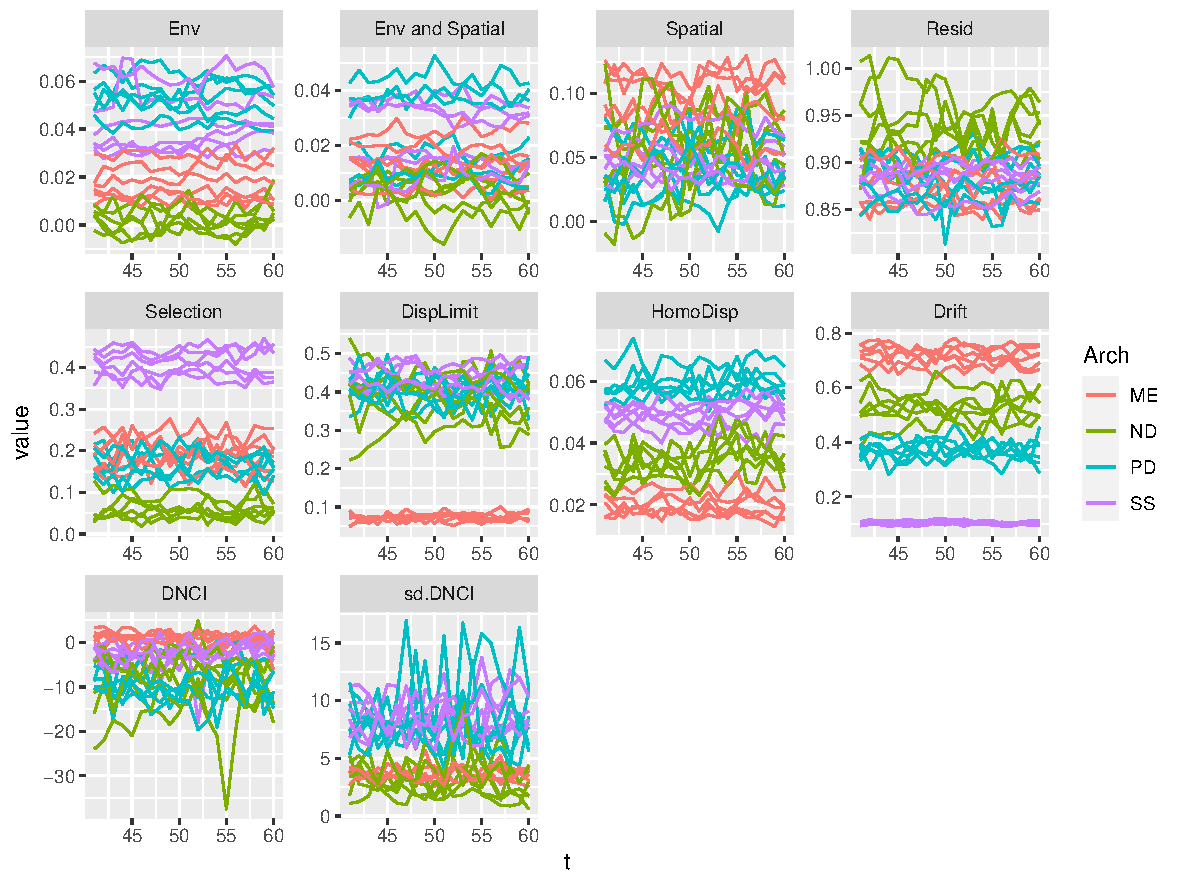
\includegraphics[width=\textwidth]{./figures/Compare_archetypes_six_rep.pdf}
	\caption[Comparing the dynamics of the summary statistics derived by beta-diversity variation partitioning, Stegen's framework and DNCI under four metacommunity archetypes.]{\small
		Comparing the dynamics of the summary statistics derived by beta-diversity variation partitioning, Stegen's framework and DNCI under four metacommunity archetypes. Within each panel, the curve shows the dynamics of the values of each summary statistic across time. The first row shows the dynamics of the variation explained only by the environment [a], by both environment and space [b], only by space [c], and unexplained variation [d] derived from beta diversity variation partitioning. The second row shows the dynamics of the fraction of selection, dispersal limitation, homogenizing dispersal, and drift derived from Stegen's framework. The third row shows the dynamics of DNCI and its standard deviation. Different colors represent different metacommunity archetypes. A maximum of six replicates are shown for each archetype.}
	\label{fig:stat_comp}
\end{figure}

% table: Overview of the summary statistics
\afterpage{
	\begin{footnotesize}
		% table: performance
		\setlength\tabcolsep{1.5pt}
		\begin{longtable}{l|rrrrrrrrrr}
			\caption[Overview of all statistics derived by beta-diversity variation partitioning, Stegen's framework and DNCI]{\small
				Overview of all statistics derived by beta-diversity variation partitioning, Stegen's framework and DNCI. For the description of the statistics please see the caption of Fig. \ref{fig:stat_comp}.}
			\label{tbl:sum_stat}
			\endfirsthead
			\toprule
			\multicolumn{1}{l}{} & \multicolumn{4}{c}{Stegen} & \multicolumn{4}{c}{VP} &  &  \\ 
			\cmidrule(lr){2-5} \cmidrule(lr){6-9}
			\multicolumn{1}{l}{} & Selection & DispLimit & HomoDisp & Drift & Env & Env and Spatial & Spatial & Resid & DNCI & sd.DNCI \\ 
			\midrule
			Min & 0.00 & 0.00 & 0.00 & 0.04 & -0.01 & -0.09 & -0.16 & 0.14 & -383.48 & 0.02 \\ 
			Max & 0.78 & 0.94 & 0.66 & 0.99 & 0.64 & 0.51 & 0.43 & 1.16 & 298.89 & 146.72 \\ 
			Mean & 0.15 & 0.27 & 0.05 & 0.53 & 0.07 & 0.05 & 0.06 & 0.82 & -7.60 & 2.31 \\ 
			Sd & 0.18 & 0.22 & 0.05 & 0.28 & 0.09 & 0.07 & 0.05 & 0.18 & 15.00 & 3.43 \\ 
			\bottomrule
		\end{longtable}
	\end{footnotesize}
}
%


\section{Performance in prediction model parameters}
\noindent
The accuracy in predicting the process parameters was quantified for all 12 random forests (RFs) (Tab. \ref{tbl:rf}). Among 12 RFs, the one that embedded all statistics of 20 snapshots had the highest accuracy in predicting dispersal ability (71.92\%) and niche width (72.02\%). This RF also had the second-highest accuracy in predicting competition type (87.49\%), which was only 0.31\% less than the RF with the highest accuracy. The second best RF was the one with all summary statistics at four snapshots as the explanatory variables, which had 68.61\%, 71.97\% and 87.80\% correction rates in predicting the dispersal ability, niche width and competition type, respectively. For the RFs that only considered one analytical method, Stegen's framework had the highest accuracy in predicting all three model parameters compared to beta-diversity variation partitioning and DNCI with the same number of snapshots. However, the RFs which integrated statistics derived from multiple analytical methods had better accuracy than those which only considered statistics derived from single analytical methods in predicting the model parameters.

The importance of the explanatory variables of the RF that incorporates the summary statistics derived from three different analytical methods based on the four snapshots was quantified (Tab. \ref{tbl:impo}). The fraction of homogenizing dispersal and selection derived from Stegen's framework and the standard deviation of DNCI were the most three important statistics for predicting the competition type. The fraction of selection, homogenizing dispersal and dispersal limitation derived from Stegen's framework and the variation explained by space derived from variation partitioning were the most important statistics for predicting dispersal ability. Variation explained only by environment, the fraction of selection and drift derived from Stegen's framework were the most important statistics for predicting niche width.

%
%

\section{Robustness to the sampling effort and choice of time steps}
\noindent
For the trained RF with summary statistics derived by three analytical methods from four snapshots, the accuracy for predicting the niche width, dispersal ability and competition type decreased when the sampling effort decreased (Fig. \ref{fig:robust-samp}). However, the accuracy for predicting the dispersal ability, niche width and competition type had no difference even though the summary statistics were derived from the species composition at four randomly selected time steps (Fig. \ref{fig:robust-time}). 

\begin{figure}
	\centering
	\begin{subfigure}[b]{0.47\textwidth}
		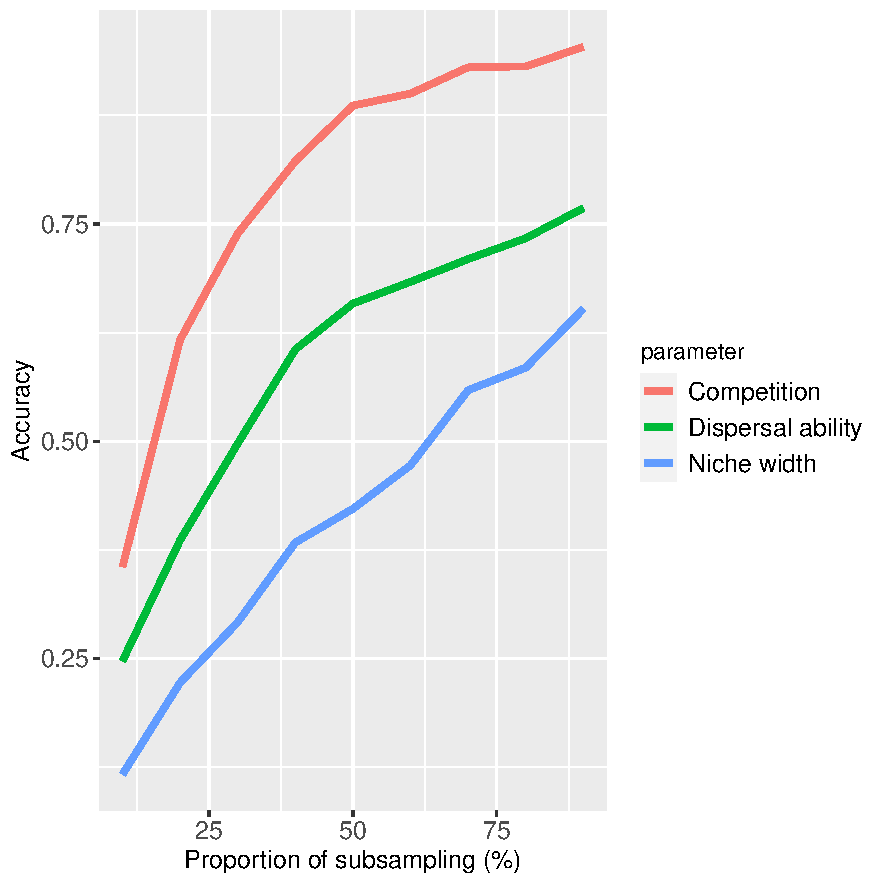
\includegraphics[width=\textwidth]{./figures/Robustness_sampling_effort_Accuracy.pdf}
		\caption{Sampling effort}
		\label{fig:robust-samp}
	\end{subfigure}
	\begin{subfigure}[b]{0.47\textwidth}
		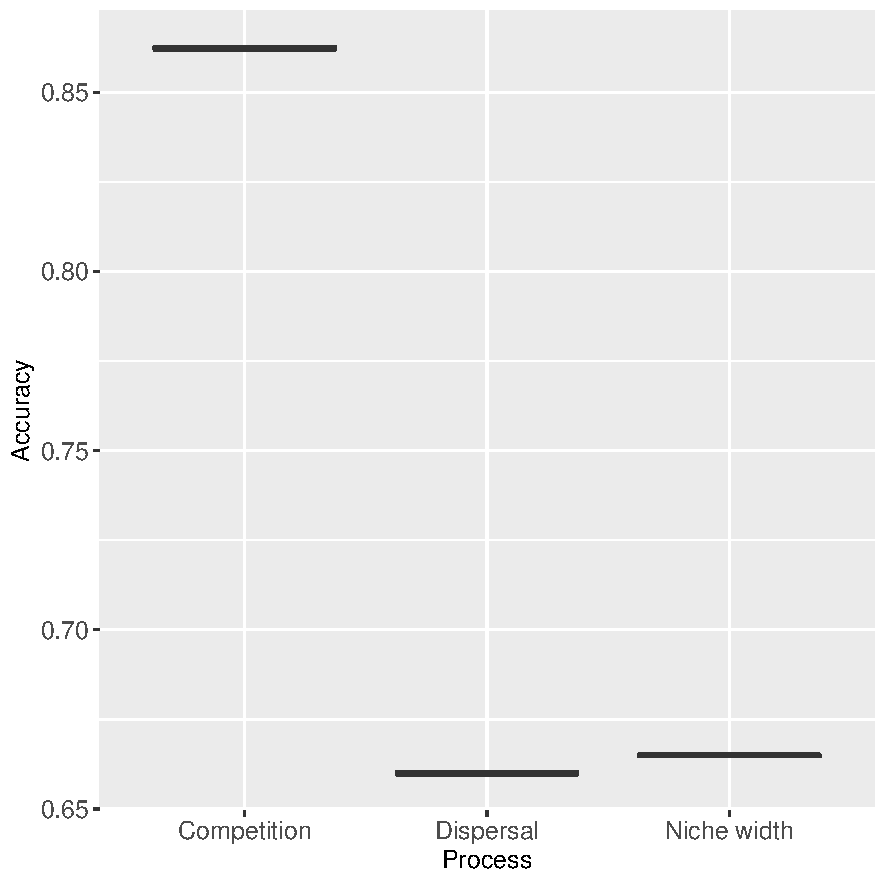
\includegraphics[width=\textwidth]{./figures/Robustness_time_step_Accuracy_distribution.pdf}
		\caption{Choice of time steps}
		\label{fig:robust-time}
	\end{subfigure}
	\caption[Robustness of random forest to the sampling effort and choice of the time steps.]{\small
		Robustness of random forest (RF) to the sampling effort and choice of the time steps. (a) Different curves represent the relationship between the accuracy for predicting competition type, niche width and dispersal ability, and proportion of the subsampled patches from a whole simulated metacommunity. (b) The distribution of the accuracy of the RF for predicting competition type, niche width and dispersal ability when using the summary statistics at the randomly chosen time steps. The variance of the accuracy is considerably small that is not visible in the boxplots displayed.}
	\label{fig:robust}
\end{figure}
%

% table: performance
\afterpage{%
	\begin{small}
		\begin{longtable}{lrrrrrrrrrr}
			\caption[Accuracy of 12 RFs with different explanatory variables in prediction model parameters.]{\small
				Accuracy of 12 RFs with different explanatory variables in prediction model parameters. The first four columns show the explanatory variables in the RFs. The symbol "O" represents the summary statistics derived from which analytical methods are considered in the RF. The symbol "X" represented they are not considered in the RF. The fourth column represented how many snapshots of the species composition are used to calculate the summary statistics and considered as the explanatory variables in the RF. The accuracy for predicting dispersal ability, niche width and competition type is shown in the last 3 columns. VP: beta-diversity variation partitioning. Stegen: Stegen's framework. DNCI: DNCI and its standard deviation.}
			\label{tbl:rf}
			\endfirsthead
			\toprule
			\multicolumn{4}{c}{Explanatory variables} &  &  &  \\ 
			\cmidrule(lr){1-4}
			\multicolumn{3}{c}{Summary statistics} &  & \multicolumn{3}{c}{Performance of prediction} \\ 
			\cmidrule(lr){1-3} \cmidrule(lr){5-7}
			VP & Stegen & DNCI & Snapshots & Dispersal ability & Niche width & Competition type \\ 
			\midrule
			O & X & X & 1 & 18.83\% & 42.59\% & 45.86\% \\ 
			O & X & X & 4 & 21.95\% & 50.83\% & 56.40\% \\ 
			O & X & X & 20 & 24.01\% & 52.13\% & 60.32\% \\ 
			X & O & X & 1 & 45.10\% & 46.91\% & 69.46\% \\ 
			X & O & X & 4 & 53.14\% & 53.74\% & 77.00\% \\ 
			X & O & X & 20 & 57.36\% & 53.24\% & 78.96\% \\ 
			X & X & O & 1 & 18.08\% & 23.96\% & 45.76\% \\ 
			X & X & O & 4 & 26.27\% & 29.43\% & 55.80\% \\ 
			X & X & O & 20 & 30.79\% & 32.95\% & 59.87\% \\ 
			O & O & O & 1 & 61.07\% & 69.61\% & 84.43\% \\ 
			O & O & O & 4 & 68.61\% & 71.97\% & 87.80\% \\ 
			O & O & O & 20 & 71.92\% & 72.02\% & 87.49\% \\ 
			\bottomrule
		\end{longtable}
	\end{small}
}


\section{Application to Fushan Forest Dynamics Plot}
\noindent
By inputting the summary statistics derived from four snapshots of the FDP by three analytical methods (Tab. \ref{tbl:empirical}), we estimated that the species in the FDP act with competition-colonization trade-off and strong average dispersal ability and wide niche width (Fig. \ref{fig:para-CC}). 

%

\newpage
\chapter*{4. Discussions}
\setcounter{chapter}{4}
\addcontentsline{toc}{chapter}{4. Discussions}
\noindent
Multiple analytical methods were introduced to derive summary statistics from the observational data to quantify the ecological information of the observed metacommunity and disentangle the underlying ecological processes. However, a single analytical method on a snapshot of the metacommunity has unsatisfying performance in predicting the underlying processes was shown in \citet{guzman2022accounting} and confirmed in our study. Within the three analytical methods considered in our study, we showed that only Stegen's framework could successfully separate the four metacommunity archetypes, which were arbitrarily defined to represent the extreme scenarios of the simulated metacommunity (Fig. \ref{fig:stat_comp}). Even though Stegen's framework could successfully separate the four archetypes, its performance in predicting the precise underlying processes was still unsatisfying. By integrating more analytical methods applied on multiple snapshots of the metacommunity, the prediction of the underlying processes may be improved. 

RF was used to link the summary statistics derived from the analytical methods with the model parameters in a process-based simulation model. We showed that this technique successfully integrates multiple analytical methods to disentangle the ecological processes underlying the observed metacommunity in \citeauthor{guzman2022accounting}'s framework. From the application of this framework in the observational data, we showed that competition-colonization trade-off was identified among the species in the Fushan Forest Dynamics Plot (FDP). This trade-off suggests competition hierarchy and a trade-off between the ability of competition and colonization among the species. The competition hierarchy between species may indicate that the FDP is composed of early-successional and late-successional species. Late-successional species may be missing in some areas of this forest plot because of the frequent impact of typhoons during summer, which creates empty patches for the early-successional species to establish. The frequent impacts of typhoons may be also the reason for the strong stochasticity and weak deterministic effect of the environmental conditions we found in the FDP, which are indicated by the predicted wide niches of the species. Strong average dispersal ability may result in the high occurrence of the common species, e.g. \textit{Blastus cochinchinensis} (柏拉木) and \textit{Helicia formosana} (山龍眼). 

This practical demonstration is missing in \citet{guzman2022accounting}. In our study, we showed that \citeauthor{guzman2022accounting}'s framework may be applied to disentangle the ecological processes underlying the observed metacommunity by plotting it onto the parametric space. However, several issues need to be considered.

First, the assumptions of the process-based simulation model should align with the observed metacommunity. In our study, \citeauthor{thompson2020process}'s metacommunity simulation model considers species as annual plants that die in each iteration, which may not correctly represent the long-living woody plant species in the FDP. The impact of this mismatch on the results is unknown and requires further investigation. Additionally, we assumed constant environmental conditions in our simulated metacommunity over time. This assumption may not be satisfied for the marine and tidal ecosystems whose environmental conditions in the local communities are intensively fluctuating. Furthermore, we assumed all the species had the same niche width and dispersal ability. To release this assumption for modeling a more complex system, we may assume that the niche width and the dispersal ability of the species are followed normal distributions with adjustable mean and variance. Since the model assumptions and the parametric space are determined before the simulation and construction of the RFs, any changes are expected to influence the parameter estimation and its accuracy. Hence, the accuracy of the RF in predicting the model parameters may not be compared across process-based simulation models with different model assumptions and parametric spaces.

Second, the process-based simulation model should generate a relatively complete range of summary statistics. Any statistics which can be derived from both simulated data and observed data could be the explanatory variables in the RF. However, if the statistics calculated by the observed data are not encompassed within the extent that the simulation model can generate, the prediction may be unreasonable. In our study, the determined parametric space in the simulation model generated a relatively complete range of summary statistics derived from the three analytical methods. Moreover, the summary statistics calculated by the observational data from the FDP were encompassed within the range of summary statistics. In \citet{guzman2022accounting}, the descriptive statistics were included as the explanatory variables of the RF. However, some of the descriptive statistics are intensively varied across systems and may not be easily controlled in the process-based simulation model. For example, gamma diversity is one of the descriptive statistics of the metacommunity. It may not only be regulated by the strength of ecological processes, but also by the size of the species pool and the number of patches of the simulated metacommunity. Without modifying these two parameters in our study, the range of the gamma diversity derived from the simulated data would be limited and may not encompass the gamma diversity derived from the observed metacommunity. 

Third, the incompleteness of the observed data may influence the accuracy of parameter estimation. We showed that the incompleteness of the species composition reduced the performance of the trained RF in predicting the model parameters. In practice, because of the variety of functional responses and resource types, we can never measure all types of traits and environmental variables. This incompleteness of the community data may cause deviation in summary statistics. For example, the unmeasured environmental variables are shown to considerably influence the summary statistics of the beta-diversity variation partitioning \citep{chang2013better}. We expect this deviation may lead to the performance of the trained RF being overestimated. The magnitude of the deviation is determined by the robustness of the analytical methods themselves. Thus, the robustness of the analytical methods should be compared systematically, and the summary statistics that are too sensitive to the incompleteness of the data should be excluded from the set of explanatory variables.

Fourth, the choice of the time steps to calculate the summary statistics as the explanatory variables of the RF may influence the parameter estimation. The simulation models are likely to generate more snapshots of the species composition than is usually available for observed data. The training data of the RF is determined by the summary statistics calculated by the simulated data at the arbitrarily chosen time steps. Moreover, the number of the chosen time steps should be identical to the census times of the observed metacommunity. However, in practice, we usually do not know which time steps in the simulation model represent which census of the observed metacommunity. We showed that even though the time steps to calculate the statistics as the inputs of the RF were randomly chosen, the performance of the RF was maintained. If the summary statistics have no stable trends across time, we expect that the choice of the time steps may influence the parameter estimation, and such statistics should be excluded from the explanatory variables of the RF.

\chapter*{5. Future Directions}
\setcounter{chapter}{5}
\addcontentsline{toc}{chapter}{5. Future Directions}
\noindent
We demonstrated \citeauthor{guzman2022accounting}'s framework in disentangling the ecological processes underlying the observed metacommunity. In practice, the process-based simulation model can be modified or replaced based on different focuses on the ecological processes and different types of ecosystems. \citeauthor{thompson2020process}'s model is principally based on high-level ecological processes and is sufficiently general to be applied to different community systems. By modeling more detailed ecological processes, e.g. how seed germination and variation in the mortality rate in seedling and juvenile stage would influence the colonization of the species or releasing the assumption of identical niche width and dispersal ability of the species, we may understand more about under what processes allow different species assemble to become a community and metacommunity. However, the trade-off between generality, realism, and precision cannot be ignored \citep{levins1966strategy}. Constructing a comprehensive and complex process-based model may result in losing its generality to apply to different ecosystems and reduce the precision in estimating the model parameters. In this case, we should generate more training data or apply a more powerful technique for parameter estimation. Besides, the sets of analytical methods for predicting the strength of ecological processes may be considered based on the availability of the data. For instance, if the functional traits data of the species are not available, the trait-based analytical methods, i.e. modified Stegen's framework, cannot be applied. 

Except for RF, there are also other approaches to estimate the parameters in a process-based stochastic model \citep{hartig2011statistical}. For example, approximation Bayesian computation (ABC) is a rejection algorithm for estimating the parameters in the process-based simulation model based on summary statistics \citep{csillery2010approximate}. \citet{van2015new} applied ABC to quantify the strength of limiting similarity, dispersal assembly and filtering underlying the observed metacommunities based on the functional diversity metrics. \citet{ruffley2019identifying} compared and incorporated RF and ABC to quantify the strength of competition and environmental filtering based on the information about phylogeny, functional traits and phylogenetic signals within the traits of the local community. Different statistical classifiers may be compared and incorporated to improve the performance in estimating the model parameters. Alternatively, cross-validation may be further applied to find the subset of the explanatory variables that maximize the performance.

Improving the framework for better disentangling the underlying ecological processes is essential for understanding and predicting how anthropogenic activity and climate change affect the species composition, diversity and ecosystem services. By estimating the model parameters based on the metacommunities across changes in environmental conditions, we may study how the strength of the ecological processes is altered by anthropogenic activity and climate change. We may further predict the dynamics of the metacommunity based on the process-based model with estimated model parameters to reach better principles for conservation.




\chapter*{Conclusions}
\setcounter{chapter}{6}
\addcontentsline{toc}{chapter}{Conclusions}
\noindent
\citet{guzman2022accounting} provided a framework that may integrate multiple analytical methods and multiple snapshots of the observational metacommunity to disentangle the ecological processes underlying the observed metacommunity. Our study demonstrates this framework in practice by the observational data from the Fushan forest and shows the competition-colonization trade-off among species and the strong stochasticity and dispersal ability of the species in the Fushan forest. The performance of this framework in quantifying the strength of the ecological processes may be evaluated. However, this performance may be overestimated because of the incompleteness of the observational data and the inference of this framework may be influenced by the assumptions of the process-based simulation model.


\section*{Data availability}
\noindent
All the codes may be found in: \url{https://github.com/ChingLinHuang/Code-for-Master-Thesis}.
